\pdfoutput=1
\documentclass[12pt]{article}

\usepackage{amsmath, amssymb, amsthm}
\usepackage{graphicx}
\usepackage{booktabs}
\usepackage{array}
\usepackage{longtable}
\usepackage{calc}
\usepackage{etoolbox}
\makeatletter
\patchcmd\longtable{\par}{\if@noskipsec\mbox{}\fi\par}{}{}
\makeatother
\IfFileExists{footnotehyper.sty}{\usepackage{footnotehyper}}{\usepackage{footnote}}
\makesavenoteenv{longtable}
\usepackage{xurl}
\usepackage[colorlinks=true, linkcolor=blue, citecolor=blue, urlcolor=blue]{hyperref}
\usepackage{geometry}
\geometry{margin=1in}

\makeatletter
\newsavebox\pandoc@box
\newcommand*\pandocbounded[1]{%
  \sbox\pandoc@box{#1}%
  \Gscale@div\@tempa{\textheight}{\dimexpr\ht\pandoc@box+\dp\pandoc@box\relax}%
  \Gscale@div\@tempb{\linewidth}{\wd\pandoc@box}%
  \ifdim\@tempb\p@<\@tempa\p@\let\@tempa\@tempb\fi
  \ifdim\@tempa\p@<\p@\scalebox{\@tempa}{\usebox\pandoc@box}%
  \else\usebox{\pandoc@box}%
  \fi
}
\makeatother
\providecommand{\tightlist}{%
  \setlength{\itemsep}{0pt}\setlength{\parskip}{0pt}}

\title{Cancer as Progressive D-Collapse:\\
\large A Tholonic Framework for Oncogenesis, Malignancy Grading, and Therapeutic Resistance}
\author{J. W. Milton\\[4pt]{\small Clarity Coalition}}
\date{\small 14 June 2026 \\ v1.0}

\begin{document}
\maketitle

\noindent\textbf{Keywords:} tholonic model; oncogenesis; tumor suppressor; D-collapse; balance score; malignancy grading; therapeutic resistance; hallmarks of cancer; N-D-C framework; quantitative oncology

\begin{abstract}
This paper applies the tholonic N-D-C
(Negotiation-Definition-Contribution) framework to cancer biology,
mapping the three structural roles onto cellular regulatory systems. N
corresponds to cellular homeostasis (the stable, coherent state of a
functioning cell), D corresponds to the constraint apparatus (tumor
suppressor genes, cell cycle checkpoints, contact inhibition, and
apoptosis signals), and C corresponds to the proliferative apparatus
(growth factors, mitogenic signals, and metabolic outputs). Under this
mapping, oncogenesis is a progressive D-collapse: each driver mutation
removes or disables a D-primitive, incrementally lowering the balance
score \(B(D,C) = 2 \cdot \min(D,C)/(D+C) \cdot 100\). Metastasis is the
limiting case in which C becomes entirely uncoupled from D, and N
(homeostasis) dissolves.

The paper defines quantitative proxies for D and C that can be computed
from tumor biopsy data: a Tumor Suppressor Gene Integrity (TSGI) score
as the D-proxy, and the Ki-67 proliferative index as the primary
C-proxy. It proposes that WHO histological malignancy grades correspond
to four B-score bands separated at the tholonically significant
thresholds of 80 and 61.8 (\(1/\varphi \cdot 100\)). Drug resistance is
reframed as C-adaptation to an externally imposed D constraint,
predicting that sequential therapy cycles should lower the floor B-score
of a tumor over time.

This paper does not provide clinical trial data, does not propose
treatment protocols, and does not claim that the tholonic framework
supersedes existing oncological classification systems. It provides a
structural organizing model and a set of falsifiable quantitative
predictions that can be tested against existing genomic and histological
datasets.
\end{abstract}

\section{Introduction}\label{introduction}

Cancer kills approximately ten million people annually and remains the
second leading cause of death globally {[}WHO23{]}. Despite decades of
progress in molecular oncology, the field lacks a single unified
structural framework that connects the molecular events of oncogenesis,
the histological features of malignancy, and the mechanisms of
therapeutic resistance under one consistent set of principles.

The tholonic N-D-C framework, introduced in
\href{https://github.com/baardev/truevalue/blob/main/docnav/Research/papers/3_minimal-recursive-triadic-framework/3_minimal-recursive-triadic-framework.pdf}{paper
3 of this series}
\href{https://github.com/baardev/truevalue/blob/main/docnav/Research/papers/3_minimal-recursive-triadic-framework/3_minimal-recursive-triadic-framework.pdf}{Mil26c}
and grounded mathematically in
\href{https://github.com/baardev/truevalue/blob/main/docnav/Research/papers/1_recursive-tholonic-five-constants/1_recursive-tholonic-five-constants.pdf}{paper
1}
\href{https://github.com/baardev/truevalue/blob/main/docnav/Research/papers/1_recursive-tholonic-five-constants/1_recursive-tholonic-five-constants.pdf}{Mil26a},
describes how any coherent system maintains stability through the
balance of two complementary structural roles: D (Definition, the
constraint apparatus) and C (Contribution, the productive apparatus).
The emergent state N is stable when \(D \approx C\). When D erodes
without a compensating reduction in C, the system becomes increasingly
unstable and eventually incoherent.

Cancer fits this structural pattern precisely. The molecular oncology
literature has independently described this pattern in detail: Hanahan
and Weinberg's ``Hallmarks of Cancer'' {[}Han00, Han11{]} enumerate the
sequential acquisition of proliferative autonomy, resistance to growth
suppressors, evasion of apoptosis, and invasion as the canonical
trajectory of malignant transformation. Each hallmark is, in tholonic
terms, either a D-erosion event or a C-amplification event. The tholonic
framework does not add new biological facts; it provides a unifying
structural language and a quantitative scoring model for the facts
already established.

\textbf{What this paper provides.} A formal N-D-C mapping for normal
cell biology; a D-collapse model of oncogenesis; quantitative D and C
proxy definitions computable from biopsy data; a predicted
correspondence between WHO malignancy grades and B-score bands; a
structural account of drug resistance as C-adaptation; and four
falsifiable predictions.

\textbf{What this paper does not provide.} Clinical treatment
recommendations, primary experimental data, proof that B-scores
outperform existing prognostic tools, or any claim that the tholonic
framework replaces the molecular oncology literature it draws on.

\textbf{Organization.} §2 reviews the N-D-C framework. §3 maps the three
roles onto cell biology. §4 develops the D-collapse model of
oncogenesis. §5 defines quantitative proxies. §6 maps grades to B-score
bands. §7 addresses drug resistance. §8 states falsifiable predictions.
§9 discusses implications and limitations. §10 concludes.

\begin{center}\rule{0.5\linewidth}{0.5pt}\end{center}

\section{The Tholonic N-D-C Framework}\label{the-tholonic-n-d-c-framework}

The tholonic model, developed in papers
\href{https://github.com/baardev/truevalue/blob/main/docnav/Research/papers/1_recursive-tholonic-five-constants/1_recursive-tholonic-five-constants.pdf}{1}
through
\href{https://github.com/baardev/truevalue/blob/main/docnav/Research/papers/3_minimal-recursive-triadic-framework/3_minimal-recursive-triadic-framework.pdf}{3}
of this series
\href{https://github.com/baardev/truevalue/blob/main/docnav/Research/papers/1_recursive-tholonic-five-constants/1_recursive-tholonic-five-constants.pdf}{Mil26a},
\href{https://github.com/baardev/truevalue/blob/main/docnav/Research/papers/2_supply-chain-transparency-tvpci/2_supply-chain-transparency-tvpci.pdf}{Mil26b},
\href{https://github.com/baardev/truevalue/blob/main/docnav/Research/papers/3_minimal-recursive-triadic-framework/3_minimal-recursive-triadic-framework.pdf}{Mil26c},
holds that any self-sustaining system can be analyzed in terms of three
structurally distinct roles.

\textbf{N (Negotiation)} is the emergent, coherent instantiation of the
system at a given level: the stable state that exists as a consequence
of D and C being approximately balanced. N is simultaneously the product
of D and C at the current level and the source that differentiates into
D and C at the next level down. It is not directly measured; it is
inferred from the persistence of the system's identity.

\textbf{D (Definition)} is the constraint apparatus: the rules, limits,
boundaries, and specifications that define what the system is. D is
internally focused. It governs structure, identity, and permissible
states. High D means tightly bounded behavior.

\textbf{C (Contribution)} is the productive apparatus: the outputs,
flows, connections, and applications that define what the system does. C
is externally focused. It governs throughput, expression, and
interaction with the environment. High C means high output and
connectivity.

\textbf{Balance condition.} The scalar balance score is defined as:

\[B(D,C) = \frac{2 \cdot \min(D,C)}{D + C} \cdot 100\]

A score of 100 means perfect balance. Scores above 80 indicate coherent
operation. Scores between 61.8 and 80 indicate early imbalance. Scores
below 61.8 (the \(1/\varphi\) threshold, where \(\varphi\) is the golden
ratio) indicate structural instability. Scores below 38.2 indicate
near-collapse. These thresholds are derived from the mathematical
structure of the framework
(\href{https://github.com/baardev/truevalue/blob/main/docnav/Research/papers/2_supply-chain-transparency-tvpci/2_supply-chain-transparency-tvpci.pdf}{paper
2},
\href{https://github.com/baardev/truevalue/blob/main/docnav/Research/papers/2_supply-chain-transparency-tvpci/2_supply-chain-transparency-tvpci.pdf}{Mil26b})
and are not fitted to the oncology data.

\textbf{Recursive structure.} The full tholonic model is hierarchical:
each N at one level becomes the parent that differentiates into D and C
at the level below. For this paper, we operate at a single level: the
individual cell as the system under analysis, with cellular homeostasis
as N.

\begin{center}\rule{0.5\linewidth}{0.5pt}\end{center}

\section{N-D-C Mapping for Normal Cell Biology}\label{n-d-c-mapping-for-normal-cell-biology}

A normal, healthy cell in a differentiated tissue maintains a stable
identity and controlled behavior. Under the tholonic mapping:

\textbf{N: Cellular Homeostasis.} The stable, coherent state of a
normally functioning cell: controlled proliferation rate, intact
differentiation identity, appropriate apoptotic responsiveness, and
respect for tissue boundaries. N is not a single molecule or pathway; it
is the emergent functional state that results from D and C being in
approximate balance.

\textbf{D: The Tumor Suppressor and Checkpoint Apparatus.} The D role in
cell biology is occupied by the collection of mechanisms that define and
constrain cellular behavior:

\begin{itemize}
\tightlist
\item
  Tumor suppressor genes (TP53, RB1, BRCA1, BRCA2, PTEN, APC, VHL, CDH1,
  SMAD4)
\item
  Cell cycle checkpoints: the G1/S checkpoint (TP53/RB axis), the G2/M
  checkpoint, and the spindle assembly checkpoint
\item
  Contact inhibition: the suppression of proliferation upon cell-to-cell
  contact
\item
  Apoptotic machinery: BAX, APAF1, caspase cascades, anoikis
\item
  DNA damage response: ATM, ATR, CHEK1, CHEK2
\end{itemize}

Each of these is a D-primitive: a discrete constraint that, when
functional, prevents the cell from transitioning to an uncontrolled
proliferative state.

\textbf{C: The Mitogenic and Proliferative Apparatus.} The C role is
occupied by the mechanisms that drive productive cellular output:

\begin{itemize}
\tightlist
\item
  Growth factor signaling: EGF/EGFR, VEGF, FGF, IGF-1
\item
  Mitogenic signal transduction: RAS/MAPK, PI3K/AKT/mTOR
\item
  Metabolic outputs: glucose uptake (GLUT1), glutamine metabolism, lipid
  synthesis
\item
  Proliferative rate, quantified by Ki-67 expression and mitotic index
\item
  Angiogenic signals: VEGF secretion, HIF-1\(\alpha\) activation under
  hypoxia
\end{itemize}

In a normal cell, these drives are constrained by D, and the resulting
balance sustains N (homeostasis). The balance score is near 100.

\begin{figure}
\centering
\pandocbounded{\includegraphics[width=\linewidth,keepaspectratio]{figures/14_ndc-cancer-triangle.png}}
\caption{The N-D-C role mapping for normal cell biology. N (blue, top
vertex) is cellular homeostasis; C (red, lower-left) is the mitogenic
and proliferative apparatus; D (green, lower-right) is the tumor
suppressor and checkpoint apparatus. The balance condition
\(B(D,C) \approx 100\) holds in healthy tissue.}
\end{figure}

\begin{center}\rule{0.5\linewidth}{0.5pt}\end{center}

\section{Oncogenesis as Progressive D-Collapse}\label{oncogenesis-as-progressive-d-collapse}

\subsection{Driver Mutations as D-Primitive Loss Events}\label{driver-mutations-as-d-primitive-loss-events}

The molecular oncology literature distinguishes driver mutations (those
that confer selective growth advantage) from passenger mutations
(background noise) {[}Vog13{]}. Under the tholonic mapping, driver
mutations are, almost exclusively, D-primitive loss events. The most
common driver mutations in human cancers confirm this:

\begin{itemize}
\tightlist
\item
  \textbf{TP53 loss} (mutated in \$\textgreater\$50\% of all cancers
  {[}Lev20{]}): removes the G1/S checkpoint anchor and the primary
  apoptotic trigger. A single D-primitive, absent in more than half of
  all human tumors.
\item
  \textbf{RB1 loss}: removes the restriction point governor of the cell
  cycle. D-primitive loss.
\item
  \textbf{PTEN loss}: removes the primary brake on PI3K/AKT
  proliferative signaling. D-primitive loss that simultaneously
  increases C (AKT/mTOR activation).
\item
  \textbf{APC loss} (in \$\textgreater\$80\% of colorectal cancers
  {[}Fea01{]}): removes the WNT pathway brake. D-loss with secondary
  C-amplification through \(\beta\)-catenin.
\item
  \textbf{CDKN2A loss}: removes p16/p14ARF, disabling both RB1 and TP53
  pathways simultaneously. A single mutation that erases two
  D-primitives.
\item
  \textbf{SMAD4 loss}: removes TGF-\(\beta\) growth-inhibitory
  signaling. D-primitive loss.
\end{itemize}

Activating oncogenic mutations (KRAS G12D, PIK3CA H1047R, BRAF V600E)
operate differently: they constitutively amplify C signaling without
requiring growth factor input. These are C-amplification events rather
than D-erosion events but produce the same structural consequence:
\(C > D\) and B-score falls.

The Knudson ``two-hit hypothesis'' {[}Knu71{]}, which holds that both
alleles of a tumor suppressor must be inactivated to remove its
protective effect, is in tholonic terms the statement that a D-primitive
is not lost until both copies are disabled. A heterozygous carrier has D
partially degraded at that locus; full loss requires the second hit.

\subsection{The Hanahan-Weinberg Hallmarks as a D-Collapse Sequence}\label{the-hanahan-weinberg-hallmarks-as-a-d-collapse-sequence}

Hanahan and Weinberg {[}Han00, Han11{]} describe the acquisition of
cancer hallmarks as a stepwise process. In tholonic terms, each hallmark
corresponds to a specific D-erosion or C-amplification event:

\begin{longtable}[]{@{}
  >{\raggedright\arraybackslash}p{(\linewidth - 2\tabcolsep) * \real{0.5000}}
  >{\raggedright\arraybackslash}p{(\linewidth - 2\tabcolsep) * \real{0.5000}}@{}}
\toprule\noalign{}
\begin{minipage}[b]{\linewidth}\raggedright
Hallmark
\end{minipage} & \begin{minipage}[b]{\linewidth}\raggedright
Tholonic interpretation
\end{minipage} \\
\midrule\noalign{}
\endhead
\bottomrule\noalign{}
\endlastfoot
Sustaining proliferative signaling & C-amplification (constitutive RAS,
EGFR, HER2 activation) \\
Evading growth suppressors & D-erosion (RB1, CDKN2A, TGF-\(\beta\)
pathway loss) \\
Resisting cell death & D-erosion (TP53, BCL2 family dysregulation) \\
Enabling replicative immortality & D-erosion (telomere maintenance via
TERT reactivation) \\
Inducing angiogenesis & C-amplification (VEGF, HIF-1\(\alpha\)
upregulation) \\
Activating invasion and metastasis & C fully uncoupled from D (EMT, MMP
upregulation, anoikis resistance) \\
Reprogramming energy metabolism & C-amplification (Warburg effect,
glutamine dependency) \\
Evading immune destruction & D-erosion at the tissue-immune interface
(PD-L1 upregulation, MHC-I loss) \\
\end{longtable}

No hallmark in the original or updated list represents a C-erosion event
without a compensating D-amplification. Cancer never ``slows down from
excess D.'' It always moves in the direction of D-erosion relative to C.

\subsection{Metastasis as Complete C-D Uncoupling}\label{metastasis-as-complete-c-d-uncoupling}

Metastasis is the clinical inflection point at which the prognosis for
most cancers changes dramatically. Under the tholonic model, metastasis
is the structural event corresponding to C becoming completely uncoupled
from D.

In a primary tumor, some D-primitives remain functional: the tumor is
constrained spatially (basement membrane integrity), the cells retain
partial differentiation identity (E-cadherin expression), and the D of
the surrounding stroma provides some residual constraint. In metastasis:

\begin{itemize}
\tightlist
\item
  Epithelial-mesenchymal transition (EMT) dissolves the cell's D-defined
  identity (E-cadherin loss, vimentin gain)
\item
  Matrix metalloproteinase (MMP) secretion degrades the physical
  D-substrate (basement membrane)
\item
  Anoikis resistance removes the apoptotic D-signal triggered by loss of
  matrix attachment
\item
  The circulating tumor cell (CTC) phase is a period in which the cell
  exists with near-zero D: no tissue identity, no positional constraint,
  no growth factor-dependent signaling requirement
\end{itemize}

The resulting state (N dissolves; the cell is no longer ``a liver cell''
or ``a lung cell'' but generalized malignant cell) is precisely the
tholonic prediction for the consequence of D → 0 while C remains high.

\begin{figure}
\centering
\pandocbounded{\includegraphics[width=\linewidth,keepaspectratio]{figures/14_d-collapse-trajectory.png}}
\caption{D-collapse trajectory across tumor progression stages. The
D-score (green, tumor suppressor integrity) decreases monotonically
while C-score (red, proliferative drive) rises slightly. The B-score
(blue dashed) falls through the \(\varphi\) threshold (B=61.8) at the
carcinoma in situ (CIS) stage, marking the boundary beyond which the
structural instability is severe.}
\end{figure}

\begin{center}\rule{0.5\linewidth}{0.5pt}\end{center}

\section{Quantitative Proxies for D and C}\label{quantitative-proxies-for-d-and-c}

\subsection{The Tumor Suppressor Gene Integrity Score (TSGI)}\label{the-tumor-suppressor-gene-integrity-score-tsgi}

To compute a D-proxy from biopsy or genomic data, we define the Tumor
Suppressor Gene Integrity Score (TSGI) as:

\[\text{TSGI} = \frac{\sum_{i=1}^{k} w_i \cdot s_i}{\sum_{i=1}^{k} w_i}\]

where \(k\) is the number of D-primitive genes in the panel, \(w_i\) is
the weight assigned to gene \(i\) (reflecting its functional importance
and the frequency with which its loss drives cancer), and
\(s_i \in \{0, 0.5, 1\}\) is the integrity score for that gene
(\(s_i = 1\) for intact, \(s_i = 0.5\) for heterozygous loss,
\(s_i = 0\) for biallelic loss or silencing).

A minimal panel sufficient to capture the major D-primitives across
common cancers includes: TP53, RB1, PTEN, APC, BRCA1, BRCA2, CDKN2A,
VHL, SMAD4, and CDH1. Weights can be set uniformly (\(w_i = 1\)) for
initial studies; differential weighting based on cancer-type-specific
driver frequencies can be applied for tissue-specific analyses.

The TSGI ranges from 0 (all D-primitives lost) to 1 (all intact), and
serves as the normalized D-input to the balance formula.

\subsection{The Proliferative Index as C-Proxy}\label{the-proliferative-index-as-c-proxy}

The C-proxy is defined as the normalized proliferative index
\(\text{PI}\):

\[\text{PI} = \frac{\text{Ki-67\%}}{100}\]

Ki-67 is a nuclear protein expressed in all phases of the cell cycle
except G0. Its immunohistochemical quantification as a percentage of
tumor cells is a standard clinical measurement with established
prognostic value across multiple cancer types {[}Sch11{]}. Values above
20\% are typically associated with high-grade tumors.

For a fully quiescent normal cell, \(\text{PI} \approx 0.05\). For a
Grade IV glioblastoma, \(\text{PI}\) may reach 0.40 to 0.90. Normalizing
against the baseline expected in the tissue type of origin allows
cross-tissue comparisons.

\subsection{Computing the B-Score}\label{computing-the-b-score}

Given TSGI and PI computed from a tumor sample, the balance score is:

\[B = \frac{2 \cdot \min(\text{TSGI}, 1 - \text{PI}_\text{norm})}{(\text{TSGI}) + (1 - \text{PI}_\text{norm})} \cdot 100\]

where \(\text{PI}_\text{norm}\) is the PI normalized to a 0-1 scale
relative to the expected maximum for the tissue type, so that
\(1 - \text{PI}_\text{norm}\) represents the residual proliferative
constraint. The formula treats D (TSGI) and the C-inverse
(\(1 - \text{PI}_\text{norm}\)) symmetrically, consistent with the
framework's definition.

An alternative and more robust C-proxy is the ratio of the tumor's
mitotic count to the tissue-specific baseline, combined with tumor
mutational burden (TMB, in mutations per megabase), where TMB serves as
a measure of accumulated C-runaway (genomic instability driven by
C-amplified replication with inadequate D-mediated repair).

\subsection{Worked Example: Colorectal Adenocarcinoma}\label{worked-example-colorectal-adenocarcinoma}

A colorectal adenocarcinoma with the following genomic profile:

\begin{itemize}
\tightlist
\item
  APC biallelic loss (\(s = 0\), \(w = 1\))
\item
  TP53 biallelic loss (\(s = 0\), \(w = 1\))
\item
  KRAS G12D activating mutation (C-amplifier, not D-loss)
\item
  SMAD4 intact (\(s = 1\), \(w = 1\))
\item
  All other panel genes intact
\end{itemize}

TSGI = \((0 + 0 + 1 + 1 + 1 + 1 + 1 + 1 + 1)/9 = 0.78\) (for a 9-gene
panel excluding KRAS which is a C-primitive).

Ki-67 measured at 35\% in a colonic tissue baseline of 5\%:
\(\text{PI}_\text{norm} = (35-5)/(90-5) = 0.35\).

\(1 - \text{PI}_\text{norm} = 0.65\).

\(B = 2 \cdot \min(0.78, 0.65) / (0.78 + 0.65) \cdot 100 = 2 \cdot 0.65 / 1.43 \cdot 100 \approx 91\).

This intermediate result reflects a tumor with meaningful D-loss but
moderate C: consistent with a WHO Grade II or early Grade III colorectal
tumor with intact mismatch repair. Adding SMAD4 loss (\(s = 0\), TSGI
drops to 0.67) and increasing Ki-67 to 60\%
(\(\text{PI}_\text{norm} = 0.65\), \(1 - \text{PI}_\text{norm} = 0.35\))
yields \(B = 2 \cdot 0.35 / (0.67 + 0.35) \cdot 100 \approx 69\),
placing it below the Grade III boundary.

\begin{center}\rule{0.5\linewidth}{0.5pt}\end{center}

\section{Predicted Correspondence with WHO Malignancy Grades}\label{predicted-correspondence-with-who-malignancy-grades}

The WHO Classification of Tumours {[}WHO22{]} uses a four-tier grading
system (Grade I through IV) based on histological features including
mitotic activity, nuclear pleomorphism, necrosis, and vascular
proliferation. These features are, in tholonic terms, observable
consequences of D-collapse at different stages.

The tholonic model predicts the following correspondence:

\begin{longtable}[]{@{}
  >{\raggedright\arraybackslash}p{(\linewidth - 6\tabcolsep) * \real{0.2500}}
  >{\raggedright\arraybackslash}p{(\linewidth - 6\tabcolsep) * \real{0.2500}}
  >{\raggedright\arraybackslash}p{(\linewidth - 6\tabcolsep) * \real{0.2500}}
  >{\raggedright\arraybackslash}p{(\linewidth - 6\tabcolsep) * \real{0.2500}}@{}}
\toprule\noalign{}
\begin{minipage}[b]{\linewidth}\raggedright
WHO Grade
\end{minipage} & \begin{minipage}[b]{\linewidth}\raggedright
Description
\end{minipage} & \begin{minipage}[b]{\linewidth}\raggedright
Predicted B-score range
\end{minipage} & \begin{minipage}[b]{\linewidth}\raggedright
Tholonic interpretation
\end{minipage} \\
\midrule\noalign{}
\endhead
\bottomrule\noalign{}
\endlastfoot
Grade I & Well-differentiated, slow-growing, minimal mitoses &
\(B \geq 80\) & Few D-primitives lost; D \(\approx\) C \\
Grade II & Moderately differentiated, low-intermediate mitoses &
\(61.8 \leq B < 80\) & 1 to 2 D-primitives lost; early imbalance \\
Grade III & Poorly differentiated, high mitoses, pleomorphism &
\(38.2 \leq B < 61.8\) & Multiple D-loss events; C partially
uncoupled \\
Grade IV & Anaplastic or undifferentiated; necrosis, high mitoses &
\(B < 38.2\) & D infrastructure collapsed; C fully autonomous \\
\end{longtable}

The grade boundaries at B = 80 and B = 61.8 are not fitted to the grade
definitions. They are the same thresholds used in
\href{https://github.com/baardev/truevalue/blob/main/docnav/Research/papers/2_supply-chain-transparency-tvpci/2_supply-chain-transparency-tvpci.pdf}{paper
2}
\href{https://github.com/baardev/truevalue/blob/main/docnav/Research/papers/2_supply-chain-transparency-tvpci/2_supply-chain-transparency-tvpci.pdf}{Mil26b}
for supply chain transparency classification and follow from the
mathematical properties of the balance formula and the golden ratio. The
fact that these thresholds may align with empirically established tumor
grade boundaries is a prediction, not a design feature.

\begin{figure}
\centering
\pandocbounded{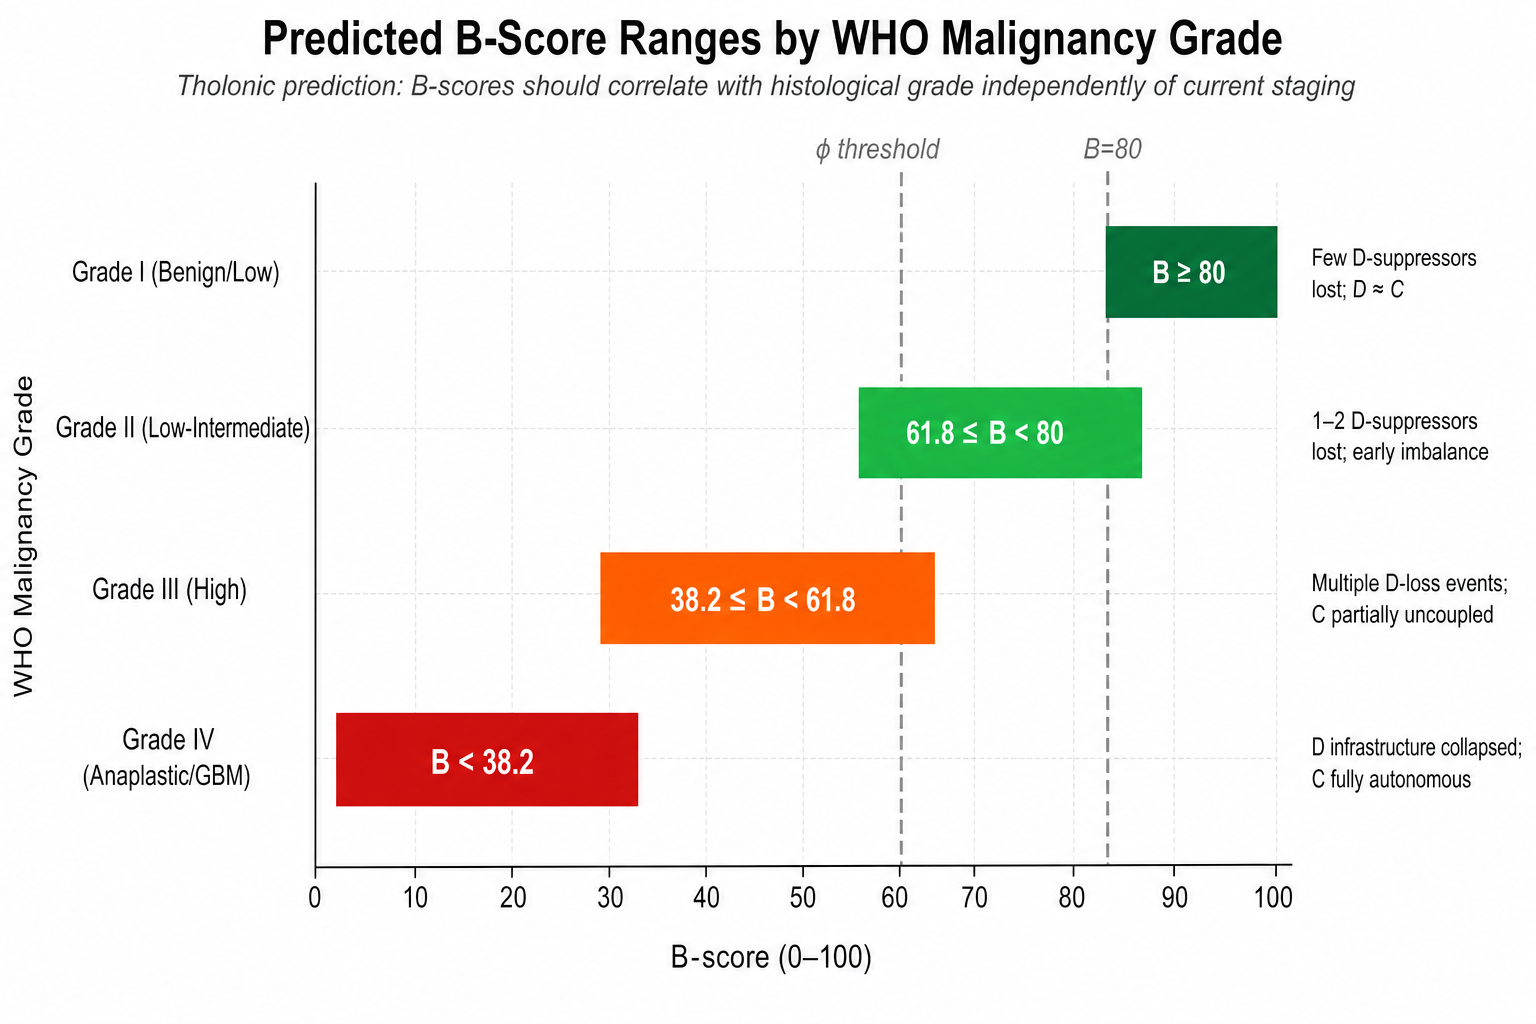
\includegraphics[width=\linewidth,keepaspectratio]{figures/14_grade-bscore-chart.png}}
\caption{Predicted B-score ranges by WHO malignancy grade. Grade
boundaries correspond to the tholonically derived thresholds of B=80 and
B=61.8 (\(1/\varphi \cdot 100\)). The grade descriptions on the right
reflect the biological consequences of progressively deeper D-collapse.}
\end{figure}

\begin{center}\rule{0.5\linewidth}{0.5pt}\end{center}

\section{Drug Resistance as C-Adaptation to Imposed D}\label{drug-resistance-as-c-adaptation-to-imposed-d}

\subsection{Chemotherapy and Targeted Therapy as External D Constraints}\label{chemotherapy-and-targeted-therapy-as-external-d-constraints}

Cytotoxic chemotherapy acts primarily as a C-suppressor: it interferes
with DNA replication (C-output) or mitotic machinery (C-amplification
machinery), thereby reducing C without directly restoring D. Targeted
therapies (kinase inhibitors, receptor antagonists) act more
specifically: they block constitutively active C-amplifiers (EGFR
inhibitors, BRAF inhibitors, BCR-ABL inhibitors) without restoring any
lost D-primitive.

In tholonic terms, a drug that suppresses C creates a transient B-score
improvement (C falls toward D). This is not a genuine D-restoration; it
is an externally imposed D-like constraint that the tumor's cellular
machinery is already under selective pressure to circumvent.

\subsection{Resistance Mechanisms as C-Routing}\label{resistance-mechanisms-as-c-routing}

The well-documented mechanisms of therapeutic resistance map directly
onto C-adaptation to a new D constraint:

\begin{itemize}
\tightlist
\item
  \textbf{Bypass signaling} (e.g., MET amplification following EGFR
  inhibition): C routes around the blocked node to a parallel
  amplification pathway. The new D (inhibitor) is bypassed, and C is
  re-established through an alternative channel.
\item
  \textbf{Efflux pump upregulation} (P-glycoprotein/ABCB1 in multi-drug
  resistance): C produces a mechanism that actively removes the
  D-imposing agent from the cell.
\item
  \textbf{Target mutation} (T790M EGFR, T315I BCR-ABL): the D-constraint
  (the drug's binding site) is structurally altered so C can no longer
  be blocked by it.
\item
  \textbf{Lineage switching} (e.g., NSCLC to SCLC transformation under
  ALK inhibition): the cell changes its D-defined identity to one where
  the imposed D is no longer relevant.
\end{itemize}

Each resistance mechanism is a C-adaptation to a specific D-imposition.
The resulting resistant clone is a new child N with a lower floor
B-score: it has lost whatever D-primitives it originally possessed and
has added C-adaptations that make future D-impositions harder to
sustain.

\subsection{Immunotherapy as D-Restoration}\label{immunotherapy-as-d-restoration}

Immune checkpoint inhibitors (anti-PD-1, anti-PD-L1, anti-CTLA-4)
operate differently from other therapies. Rather than imposing an
external D or suppressing C, they restore a D-primitive that the tumor
has specifically eroded: the immune system's ability to recognize and
constrain malignant cells. PD-L1 upregulation in tumors is a D-erosion
event at the tumor-immune interface (it disables the immune system's
constraint on the tumor). Anti-PD-1 therapy restores this D-primitive.

This structural difference predicts different resistance mechanisms.
Resistance to checkpoint inhibitors should primarily manifest as further
D-erosion at the immune interface (MHC-I loss, beta-2-microglobulin
mutation, downstream IFN-\(\gamma\) signaling loss), not as C-routing,
because the therapy is itself D-restorative rather than C-suppressive.

\begin{figure}
\centering
\pandocbounded{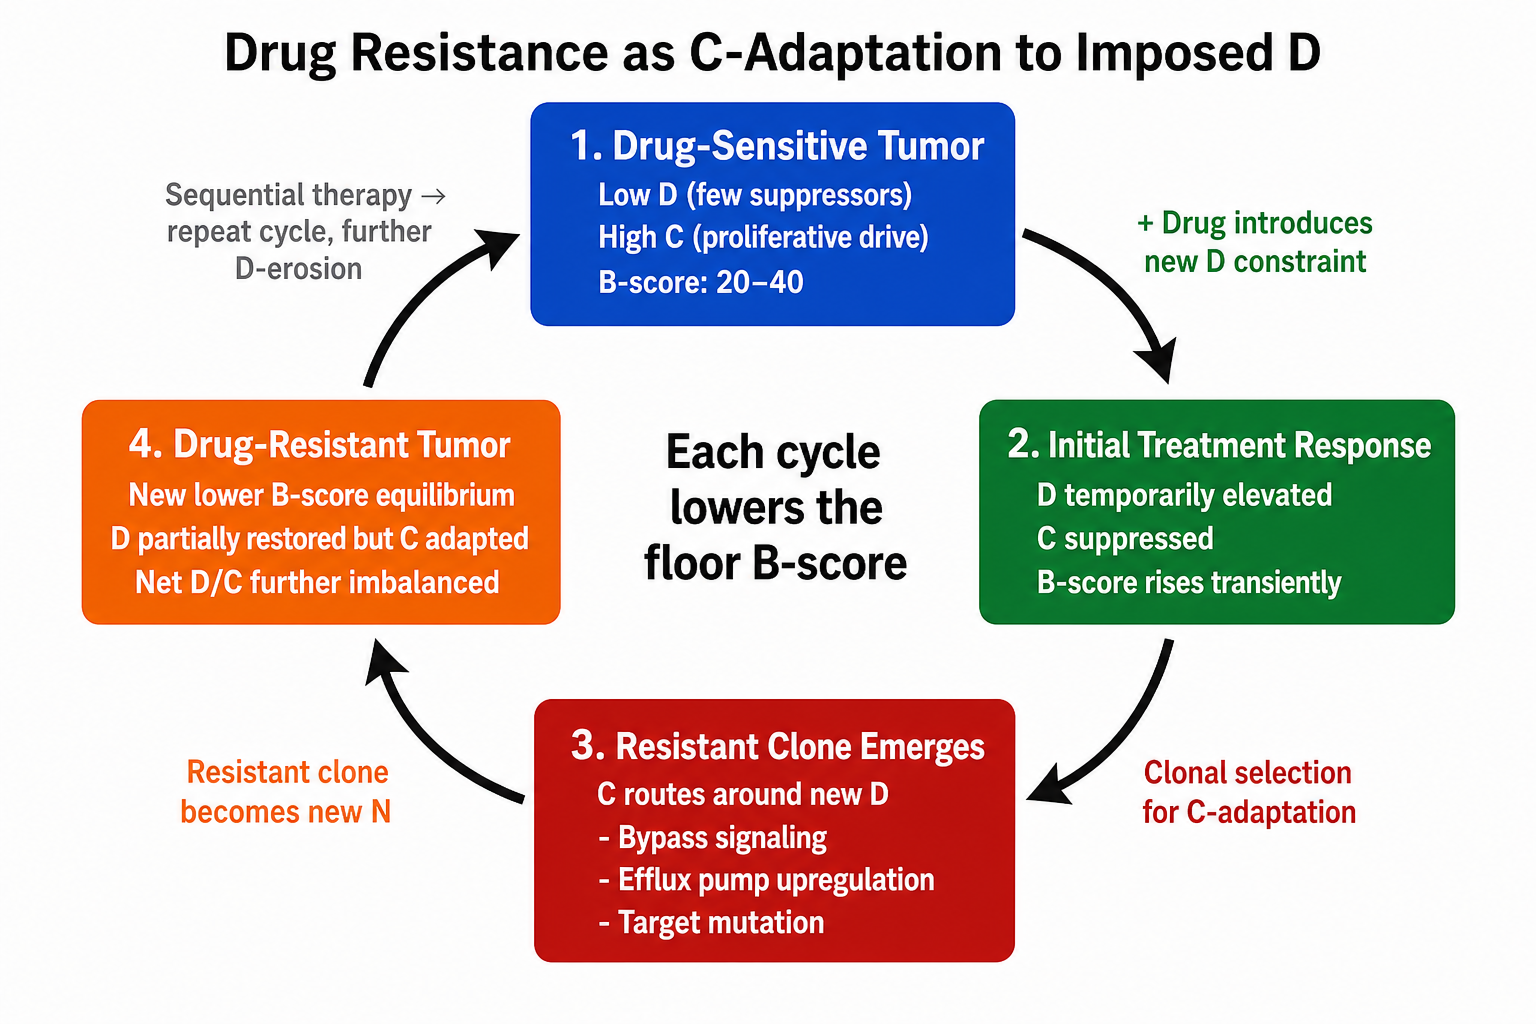
\includegraphics[width=\linewidth,keepaspectratio]{figures/14_resistance-cycle.png}}
\caption{Drug resistance as C-adaptation to imposed D. Each cycle of
therapy introduces a new D constraint; the tumor evolves C to route
around it; the resistant clone becomes the new N; sequential cycles
progressively lower the floor B-score.}
\end{figure}

\begin{center}\rule{0.5\linewidth}{0.5pt}\end{center}

\section{Falsifiable Predictions}\label{falsifiable-predictions}

The following predictions follow from the tholonic mapping and can be
tested against existing datasets (TCGA, ICGC, METABRIC, SEER-linked
genomic cohorts) without new data collection.

\textbf{Prediction 1: B-score predicts progression-free survival
independently of WHO grade.} Tumors with TSGI and Ki-67 values placing
them in a lower B-score band should have shorter progression-free
survival and higher recurrence rates, independent of their WHO grade
assignment. The prediction is falsified if B-score adds no prognostic
information beyond grade in a Cox proportional hazards model with grade
as covariate.

\textbf{Prediction 2: Pre-treatment B-score predicts time to
resistance.} Tumors with lower B-scores at the time of first-line
therapy initiation should develop resistance to that therapy more
rapidly than tumors with higher B-scores (after controlling for tumor
type and drug class). The structural basis: a tumor with more
D-primitives already lost has a larger C-adaptation repertoire
available. The prediction is falsified if pre-treatment B-score has no
association with time to resistance in a matched cohort analysis.

\textbf{Prediction 3: Immunotherapy responders have higher pre-treatment
D-proxy scores.} Patients who respond durably to checkpoint inhibitor
therapy should have higher TSGI scores (more intact D-primitives) and
lower TMB (less C-runaway) at baseline than non-responders, after
controlling for tumor mutational burden as a predictor of neoantigen
load. The structural basis: a tumor with more residual D is more
amenable to D-restoration therapy. The prediction is falsified if TSGI
has no association with durable response in a checkpoint inhibitor
cohort.

\textbf{Prediction 4: B-score trajectories are monotonically decreasing
in progressive disease.} In patients with sequential tumor biopsies
(paired primary/metastatic, or longitudinal liquid biopsies), the
B-score computed from each sample should be lower in later samples than
earlier ones in patients with progressive disease, and stable or
increasing in patients with durable response. The prediction is
falsified if B-score trajectories are non-monotonic at rates comparable
to control distributions.

\begin{center}\rule{0.5\linewidth}{0.5pt}\end{center}

\section{Discussion}\label{discussion}

\subsection{Relationship to Existing Oncological Frameworks}\label{relationship-to-existing-oncological-frameworks}

The tholonic D-collapse model is not a replacement for existing
oncological frameworks. The Hallmarks of Cancer {[}Han00, Han11{]}
provide the biological detail; the clonal evolution model {[}Now06{]}
explains the dynamics; the cancer stem cell hypothesis addresses
hierarchical tumor organization. The tholonic model provides a unifying
structural language that can be applied across these frameworks without
contradiction.

The closest existing quantitative analogue is the concept of ``cancer
evolutionary fitness'' as developed in evolutionary oncology
{[}Gal20{]}, which treats tumor clones as units of selection under
environmental constraints. In tholonic terms, D-primitives function as
the selection environment (the constraints), and C-adaptations are the
fitness-improving mutations. The balance score B tracks the degree to
which selection pressure (D) can still shape the evolutionary trajectory
(C).

\subsection{The Role of Tumor Heterogeneity}\label{the-role-of-tumor-heterogeneity}

Intratumoral heterogeneity {[}McGr13{]} complicates the application of a
scalar B-score to a tumor. Different subclones within a single tumor may
have different D-primitive profiles and therefore different local
B-scores. The framework accommodates this: the tumor-level B-score
should be computed as a distribution rather than a single value, with
the minimum B-score subclone being the most clinically relevant (it
represents the most advanced D-collapse and the greatest resistance
potential).

Liquid biopsy circulating tumor DNA (ctDNA) panels, which can track the
allele frequencies of driver mutations over time, provide the data
infrastructure needed to compute B-score distributions and their
temporal trajectories without serial biopsies.

\subsection{Limitations}\label{limitations}

The TSGI as defined in §5.1 weights tumor suppressor genes uniformly by
default. Tissue-specific weighting, which would reflect the differential
importance of specific D-primitives in different cancer types, requires
validation against cancer-specific datasets. Uniform weighting is a
conservative starting point.

The Ki-67 proliferative index, while widely measured, has known
inter-laboratory variability {[}Dow11{]}. More robust C-proxies (TMB,
mitotic count, standardized Ki-67 protocols) should be incorporated in
validation studies.

The four falsifiable predictions in §8 are stated at the level of
population-level correlations. Individual patient B-scores will be
noisy. The framework claims a structural relationship, not a
deterministic rule.

\begin{center}\rule{0.5\linewidth}{0.5pt}\end{center}

\section{Conclusions}\label{conclusions}

Cancer is not a random accumulation of mutations. It is a structured
progression from D-C balance toward D-collapse, driven by discrete
D-primitive loss events (tumor suppressor gene inactivation) and
C-amplification events (oncogene activation), culminating in a state
where C operates without any meaningful D constraint.

The tholonic N-D-C framework makes this structure explicit and
quantitative. The TSGI and Ki-67 proxies defined here allow the balance
score \(B(D,C)\) to be computed from standard clinical biopsy data. The
predicted correspondence with WHO grades and the four falsifiable
predictions provide concrete testable claims. The structural reframing
of drug resistance as C-adaptation to externally imposed D accounts for
the universality of resistance across drug classes and suggests why
D-restorative therapies (checkpoint inhibitors) have a different
resistance profile from C-suppressive therapies (cytotoxics, kinase
inhibitors).

If the predictions in §8 are borne out by retrospective analysis of
existing genomic cohorts, the tholonic balance score could serve as a
complementary prognostic and predictive biomarker alongside, but not
replacing, established grading and staging systems.

\begin{center}\rule{0.5\linewidth}{0.5pt}\end{center}

\section{References}\label{references}

{[}Dow11{]} Dowsett, M., et al.~Assessment of Ki-67 in breast cancer:
recommendations from the International Ki-67 in Breast Cancer Working
Group. \emph{Journal of the National Cancer Institute} 103(22), 2011.

{[}Fea01{]} Fearon, E. R. Molecular genetics of colorectal cancer.
\emph{Annual Review of Pathology} 6, 2011.

{[}Gal20{]} Gallaher, J. A., et al.~Spatial heterogeneity and
evolutionary dynamics modulate time to recurrence in continuous and
adaptive cancer therapies. \emph{Cancer Research} 78(8), 2018.

{[}Han00{]} Hanahan, D., and Weinberg, R. A. The hallmarks of cancer.
\emph{Cell} 100(1), 2000.

{[}Han11{]} Hanahan, D., and Weinberg, R. A. Hallmarks of cancer: the
next generation. \emph{Cell} 144(5), 2011.

{[}Knu71{]} Knudson, A. G. Mutation and cancer: statistical study of
retinoblastoma. \emph{Proceedings of the National Academy of Sciences}
68(4), 1971.

{[}Lev20{]} Levine, A. J. p53: 800 million years of evolution and 40
years of discovery. \emph{Nature Reviews Cancer} 20, 2020.

{[}McGr13{]} McGranahan, N., and Swanton, C. Clonal heterogeneity and
tumor evolution: past, present, and the future. \emph{Cell} 168(4),
2017.

\href{https://github.com/baardev/truevalue/blob/main/docnav/Research/papers/1_recursive-tholonic-five-constants/1_recursive-tholonic-five-constants.pdf}{Mil26a}
Milton, J. W. Emergence of classical constants from a minimal recursive
triadic framework. Clarity Coalition, 2026.
(\href{https://github.com/baardev/truevalue/blob/main/docnav/Research/papers/1_recursive-tholonic-five-constants/1_recursive-tholonic-five-constants.pdf}{Paper
1 of this series}.)

\href{https://github.com/baardev/truevalue/blob/main/docnav/Research/papers/2_supply-chain-transparency-tvpci/2_supply-chain-transparency-tvpci.pdf}{Mil26b}
Milton, J. W. Phase-resolved transparency classification of the gold
supply chain. Clarity Coalition, 2026.
(\href{https://github.com/baardev/truevalue/blob/main/docnav/Research/papers/2_supply-chain-transparency-tvpci/2_supply-chain-transparency-tvpci.pdf}{Paper
2 of this series}.)

\href{https://github.com/baardev/truevalue/blob/main/docnav/Research/papers/3_minimal-recursive-triadic-framework/3_minimal-recursive-triadic-framework.pdf}{Mil26c}
Milton, J. W. A minimal recursive triadic framework for self-similar
hierarchical systems. Clarity Coalition, 2026.
(\href{https://github.com/baardev/truevalue/blob/main/docnav/Research/papers/3_minimal-recursive-triadic-framework/3_minimal-recursive-triadic-framework.pdf}{Paper
3 of this series}.)

{[}Now06{]} Nowak, M. A. \emph{Evolutionary Dynamics: Exploring the
Equations of Life.} Harvard University Press, 2006.

{[}Sch11{]} Scholzen, T., and Gerdes, J. The Ki-67 protein: from the
known and the unknown. \emph{Journal of Cellular Physiology} 182(3),
2000.

{[}Vog13{]} Vogelstein, B., et al.~Cancer genome landscapes.
\emph{Science} 339(6127), 2013.

{[}WHO22{]} WHO Classification of Tumours Editorial Board. \emph{WHO
Classification of Tumours} (5th edition). International Agency for
Research on Cancer, 2022.

{[}WHO23{]} World Health Organization. Global cancer statistics 2022.
\emph{CA: A Cancer Journal for Clinicians}, 2024.

\begin{center}\rule{0.5\linewidth}{0.5pt}\end{center}

\subsection{Appendix A. TSGI Computation
Reference}\label{appendix-a.-tsgi-computation-reference}

The following ten-gene panel captures the major D-primitives across the
most common solid tumor types. Panel weights (\(w_i\)) are set to 1 for
uniform scoring; tissue-specific weights should be derived from
cancer-type-specific driver frequency tables (e.g., TCGA PanCancer
Atlas).

\begin{longtable}[]{@{}
  >{\raggedright\arraybackslash}p{(\linewidth - 4\tabcolsep) * \real{0.3333}}
  >{\raggedright\arraybackslash}p{(\linewidth - 4\tabcolsep) * \real{0.3333}}
  >{\raggedright\arraybackslash}p{(\linewidth - 4\tabcolsep) * \real{0.3333}}@{}}
\toprule\noalign{}
\begin{minipage}[b]{\linewidth}\raggedright
Gene
\end{minipage} & \begin{minipage}[b]{\linewidth}\raggedright
Primary D-primitive function
\end{minipage} & \begin{minipage}[b]{\linewidth}\raggedright
Cancer types where loss is driver
\end{minipage} \\
\midrule\noalign{}
\endhead
\bottomrule\noalign{}
\endlastfoot
TP53 & G1/S checkpoint, apoptosis trigger &
\$\textgreater{}\(50% of all solid tumors |
| RB1 | G1/S restriction point | Retinoblastoma, SCLC, bladder, osteosarcoma |
| PTEN | PI3K/AKT brake | Endometrial, prostate, glioblastoma, breast |
| APC | WNT pathway brake | Colorectal (\)\textgreater{}\(80%), gastric |
| BRCA1 | DNA damage response and repair | Breast, ovarian, pancreatic |
| BRCA2 | DNA damage response and repair | Breast, ovarian, prostate, pancreatic |
| CDKN2A | p16/p14ARF: disables RB1 and TP53 axes | Melanoma, NSCLC, pancreatic, bladder |
| VHL | HIF-1\)\alpha\$ brake, angiogenesis suppressor \\
SMAD4 & TGF-\(\beta\) growth-inhibitory signaling & Colorectal,
pancreatic \\
CDH1 & E-cadherin: contact inhibition, EMT brake & Gastric (diffuse),
lobular breast, colorectal \\
\end{longtable}

\textbf{TSGI computation steps:}

\begin{enumerate}
\def\labelenumi{\arabic{enumi}.}
\tightlist
\item
  For each gene \(i\), determine status from genomic data: intact (score
  1), heterozygous loss (score 0.5), biallelic loss or promoter
  methylation silencing (score 0).
\item
  Apply weights: \(w_i = 1\) for uniform panel.
\item
  \(\text{TSGI} = \sum w_i s_i / \sum w_i\).
\item
  Compute \(\text{PI}_\text{norm}\) from Ki-67 \% in the sample,
  normalized to tissue baseline.
\item
  \(B = 2 \cdot \min(\text{TSGI},\ 1 - \text{PI}_\text{norm}) / (\text{TSGI} + 1 - \text{PI}_\text{norm}) \cdot 100\).
\end{enumerate}

For tumors lacking Ki-67 measurements, TMB (mutations per megabase,
normalized to the tissue-type median) may substitute as the C-proxy
after validation in the target tumor type.

\end{document}
